% TBA4565 module report. Compiler: pdfLaTeX (Overleaf default); bibliography: BibTeX via natbib.
\documentclass[11pt,a4paper]{article}

\usepackage[utf8]{inputenc}
\usepackage[T1]{fontenc}
\usepackage{lmodern}
\usepackage{microtype}
\usepackage[a4paper,margin=2.5cm]{geometry}
\usepackage{amsmath,amssymb}
\usepackage{graphicx}
\usepackage{booktabs}
\usepackage{tabularx}
\usepackage{array}
\usepackage{xcolor}
\usepackage{caption}
\usepackage{subcaption}
\usepackage{enumitem}
\usepackage{tikz}
\usetikzlibrary{arrows.meta,positioning,fit,calc}
\usepackage[authoryear,round]{natbib}
\usepackage{url}
\usepackage[hidelinks]{hyperref}
\usepackage[nameinlink,capitalise]{cleveref}

\graphicspath{{figures/}}
\definecolor{ntnublue}{HTML}{00509E}
\setlist{itemsep=2pt,topsep=4pt}
\captionsetup{font=small,labelfont=bf}
\setlength{\parskip}{4pt}

% Shared TikZ styles for the architecture diagrams.
\tikzset{
  box/.style={draw=ntnublue, rounded corners=2pt, fill=ntnublue!6, align=center,
    font=\footnotesize, text width=#1, minimum height=0.95cm, inner sep=3pt},
  box/.default=2.7cm,
  store/.style={box=#1, fill=white, draw=black!55},
  store/.default=2.7cm,
  flow/.style={-{Stealth[length=2mm]}, thick, black!70},
  lab/.style={font=\scriptsize, midway, fill=white, inner sep=1pt},
}

\newcommand{\code}[1]{\texttt{#1}}
\newcommand{\dg}{\ensuremath{^\circ}}
\newcommand{\siteurl}{\url{https://progrimm.github.io/TBA4565-Geomatics-Specialization-Course/}}

\title{\textbf{My GIS module}\\[4pt]
  \large Three small web GIS projects in GI science, GI systems and 3D GIS}
\author{Åmund Grimstad\\[2pt]
  \small TBA4565 Specialization Subject: GI Science and Systems\\
  \small Norwegian University of Science and Technology (NTNU), autumn 2026}
\date{30 October 2026}

\begin{document}
\maketitle

\begin{abstract}
\noindent
This report describes three small web GIS projects I built in the specialization module TBA4565 in autumn 2026, and what I learned from building them. \emph{Projection Lab} is an interactive world map that lets anyone see how the Mercator projection distorts the size of countries compared with an equal-area map. \emph{Trondheim 3D} is a 3D model of my own city, built to learn CesiumJS, with public shelters and a walking route to the nearest one. \emph{3DGS Viewer} opens 3D Gaussian splat files in the browser, built to learn how this new kind of 3D data works on the web. The three apps are published together on one website, \siteurl. The report focuses on the purpose of each project, the technologies behind it and the experience I gained, rather than on detailed numerical results.
\end{abstract}

\tableofcontents
\clearpage

\section{Introduction}\label{sec:intro}

\subsection{Background and goal}

The module covers three themes: GI science, GI systems and 3D GIS. Instead of one large project, I chose to make one small web application for each theme. Each project starts from a single question (\cref{tab:overview}), and I wanted every app to be finished and usable by others, not only by me. The three apps are therefore published together on one website, \siteurl, where a homepage links to each of them (\cref{fig:mobile} in \cref{sec:website}). The source code is in the public repository \url{https://github.com/progrimm/TBA4565-Geomatics-Specialization-Course}.

\begin{table}[htbp]
\centering
\caption{The three projects.}
\label{tab:overview}
\small
\begin{tabularx}{\textwidth}{L{2.6cm} L{1.7cm} Y}
\toprule
Project & Theme & Question \\
\midrule
Projection Lab & GI science & How much does the Mercator projection inflate the area of each country, and how does this depend on latitude? \\
\addlinespace
Trondheim 3D & GI systems & Where is the nearest public shelter in Trondheim, and how far is the walk? \\
\addlinespace
3DGS Viewer & 3D GIS & What does a 3D Gaussian splat file contain, and can it be opened and inspected in a browser without a server? \\
\bottomrule
\end{tabularx}
\end{table}

\subsection{Way of working}\label{sec:work}

I used the AI coding assistant Claude Code \citep{claudecode} in all three projects, in two different roles. In the first part of Projection Lab, it worked as a tutor: I wrote and ran the code myself, and the assistant explained concepts and pointed me to the official documentation. In the rest of the work, the assistant wrote the code, while I set the goals, chose between alternatives, reviewed the changes and checked the result in the browser.

I chose this way of working on purpose. AI assistants are becoming a normal part of software development, and I expect that working in geomatics will involve directing and reviewing such tools as much as writing code by hand. I wanted to experience GIS development from this perspective, while still learning the underlying technologies well enough to understand and check what the assistant made.

\section{Data and tools}\label{sec:data}

All data used in the projects is open, except my own splat capture in \cref{sec:p3}. \Cref{tab:data} lists the datasets, and all screenshots in this report contain data from these sources. \Cref{tab:tools} lists the main tools and libraries, and what each one is used for.

\begin{table}[!ht]
\centering
\caption{Datasets.}
\label{tab:data}
\small
\begin{tabularx}{\textwidth}{L{3.6cm} L{2.6cm} L{1.9cm} Y}
\toprule
Dataset & Source & Licence & Description \\
\midrule
Admin 0 Countries, 1:110m & Natural Earth \citep{naturalearth} & Public domain & Boundaries of 177 countries (GeoJSON, WGS 84). Used in Projection Lab. \\
\addlinespace
Public shelters (\emph{Tilfluktsrom -- offentlige}) & DSB, WFS service \citep{dsbwfs} & NLOD 2.0 & 12 shelters with number, capacity and address, in EUREF89 / UTM zone 32N. Used in Trondheim 3D. \\
\addlinespace
Walking network & OpenStreetMap, Overpass API \citep{overpass} & ODbL & Footways, paths and streets around the shelters: 164\,294 nodes and 32\,944 ways. Used in Trondheim 3D. \\
\addlinespace
Cesium World Terrain and Cesium OSM Buildings & Cesium ion & Cesium ion terms; buildings ODbL & Global terrain and OpenStreetMap buildings, streamed as needed. Used in Trondheim 3D. \\
\addlinespace
Splat files & Own capture; ``SOAR Telescope'' by L.~Cerda \citep{soar} & Not published; CC BY 4.0 & Test files for the 3DGS Viewer. The app itself ships no data. \\
\bottomrule
\end{tabularx}
\end{table}

\begin{table}[!ht]
\centering
\caption{Main tools and libraries.}
\label{tab:tools}
\small
\begin{tabularx}{\textwidth}{L{3.6cm} L{2.6cm} Y}
\toprule
Tool & Project & Function \\
\midrule
D3 (d3-geo) \citep{d3} & Projection Lab & Projects and draws the world map in the browser \\
PostgreSQL with PostGIS & Projection Lab & Stores the countries; geodesic area with \code{ST\_Area} \citep{postgis-starea} \\
GDAL ogr2ogr \citep{gdal-ogr2ogr} & Projection Lab & Imports the GeoJSON file into PostGIS \\
pyproj \citep{pyproj} and Shapely \citep{shapely} & Projection Lab & Spherical, Mercator and Eckert IV areas \\
FastAPI \citep{fastapi} & Projection Lab & Web API between the database and the map \\
Docker Compose & Projection Lab & Runs the database, the API and the web server together \\
CesiumJS \citep{cesiumjs} and Cesium ion & Trondheim 3D & 3D globe, terrain and streaming of 3D Tiles \\
proj4js & Trondheim 3D & Converts the shelters from EPSG:25832 to WGS 84 \\
Spark \citep{spark} and three.js \citep{threejs} & 3DGS Viewer & Renders Gaussian splats with WebGL \\
React, Vite & All & User interface and build \\
Vitest, pytest, ESLint & All & Unit tests and code checks \\
GitHub Actions and Pages \citep{ghpages} & All & Automatic checks and hosting of the website \\
\bottomrule
\end{tabularx}
\end{table}

\section{Projection Lab: seeing map distortion}\label{sec:p1}

\subsection{Purpose}

Most of us learned what the world looks like from Mercator maps, where Greenland appears about as large as Africa. Every flat map has to distort the round Earth somehow, but few people know how, or that other world maps make different trade-offs. Projection Lab is meant for everyday users rather than GIS experts: one world map with a slider that morphs smoothly from Mercator to Eckert IV, an equal-area projection (\cref{fig:p1-endpoints}). Watching Greenland, Canada and Russia shrink while Africa keeps its size makes the distortion visible without any formulas. Clicking a country shows how much Mercator exaggerates its area, and a short ``Method'' section explains the ideas in plain language.

\begin{figure}[htbp]
\centering
\begin{subfigure}{0.49\textwidth}
  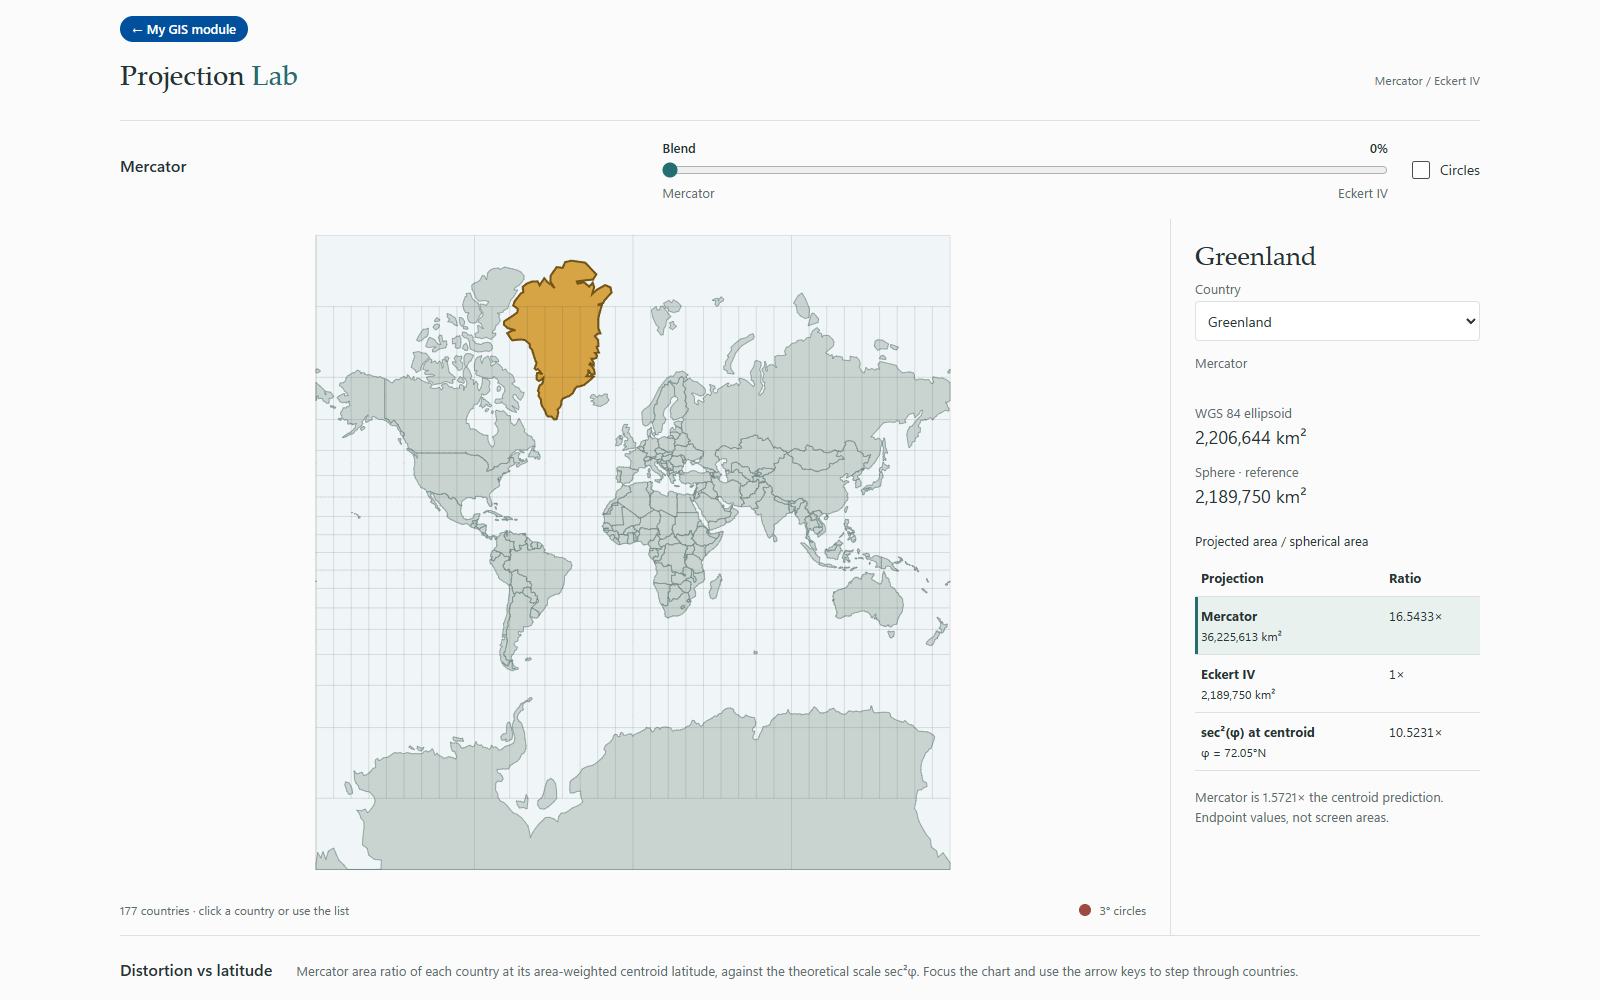
\includegraphics[width=\linewidth]{project-1-01-mercator.png}
  \caption{Mercator}
\end{subfigure}\hfill
\begin{subfigure}{0.49\textwidth}
  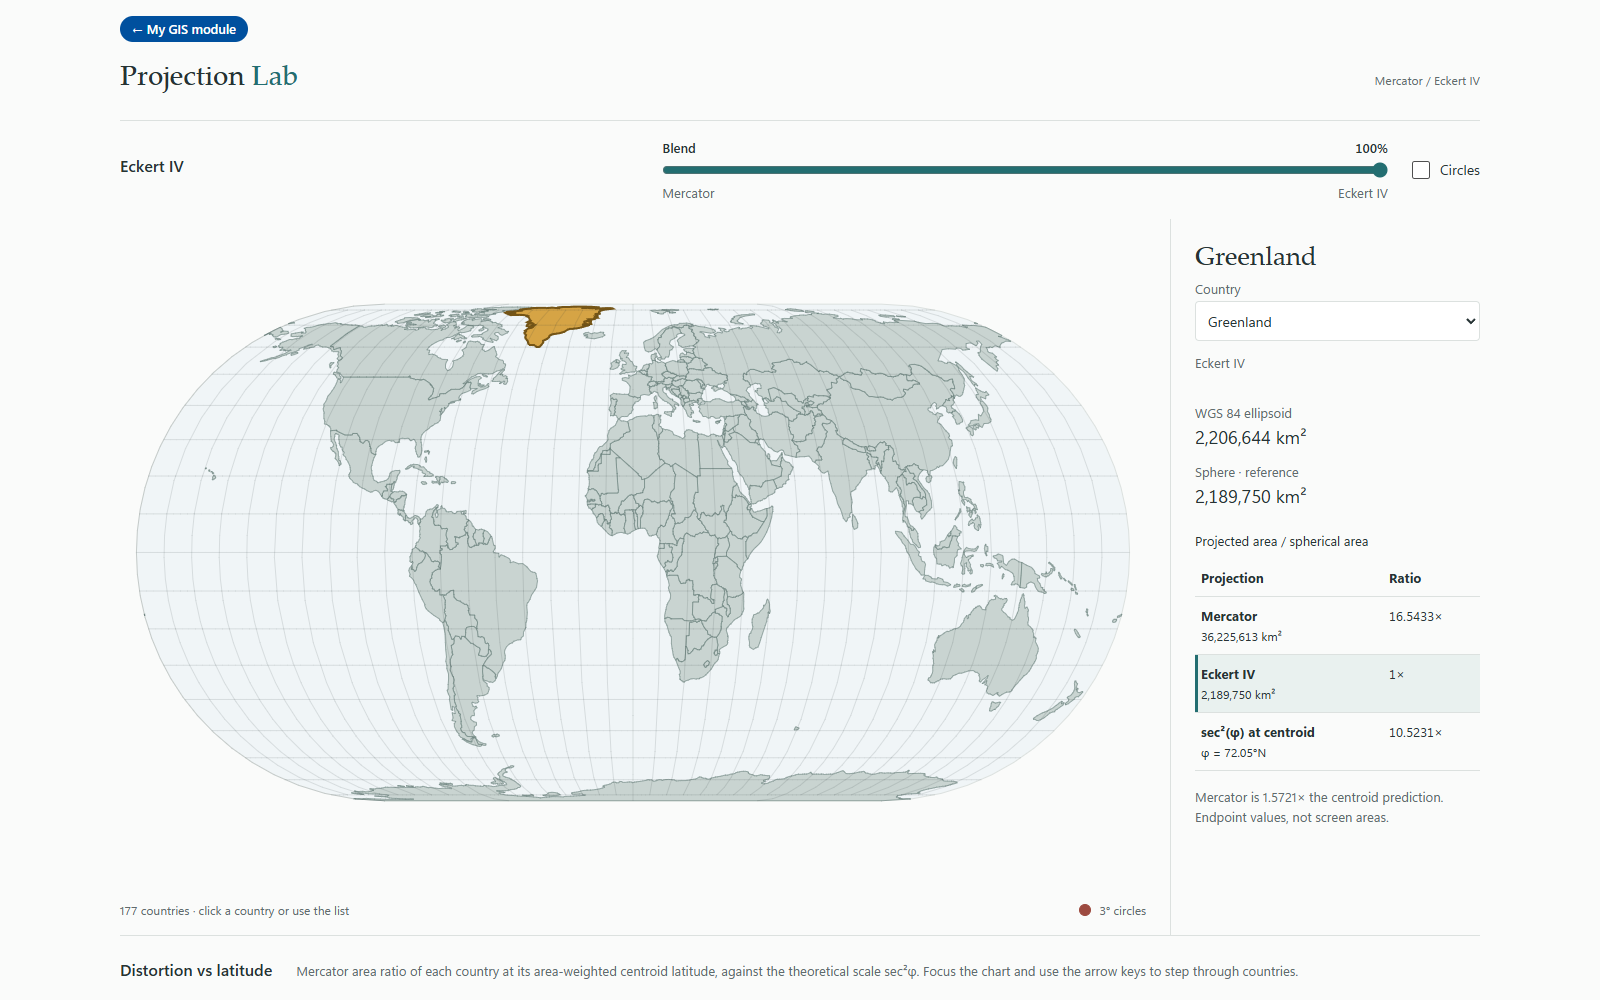
\includegraphics[width=\linewidth]{project-1-02-eckert-iv.png}
  \caption{Eckert IV (equal-area)}
\end{subfigure}
\caption{The two ends of the slider, with Greenland selected. In Mercator, Greenland is shown about 16.5 times too large; in Eckert IV it has its true relative size. Country boundaries: Natural Earth (public domain).}
\label{fig:p1-endpoints}
\end{figure}

\subsection{What I built}

\begin{itemize}
  \item A morphing world map with a blend slider, drawn in the browser with D3.
  \item Red ``distortion circles'': 30 circles of the same size on the globe, drawn through the current projection, as a simple version of Tissot's indicatrix (\cref{fig:p1-blend}). In Mercator they stay round but grow towards the poles; in Eckert IV they keep their area but get squashed.
  \item A panel for the selected country, comparing its true area with its Mercator and Eckert IV areas.
  \item A chart of distortion against latitude for all 177 countries, which shows the pattern at a glance: the farther from the equator, the larger the exaggeration.
\end{itemize}

\begin{figure}[htbp]
\centering
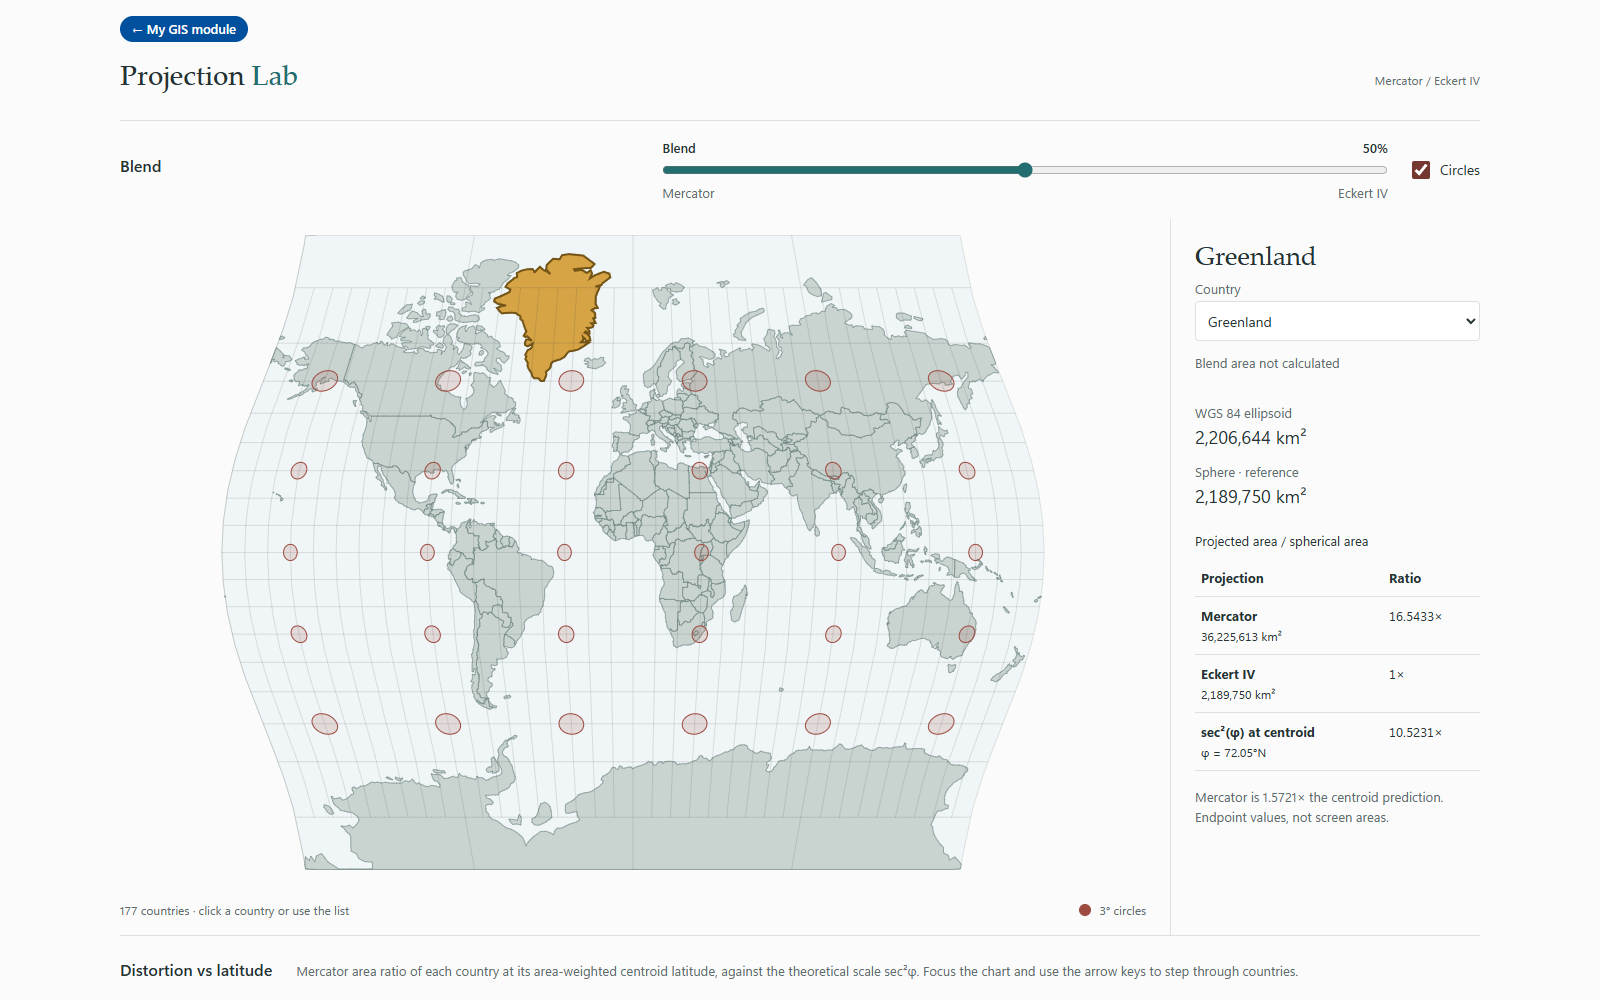
\includegraphics[width=0.8\textwidth]{project-1-03-blend-50-circles.png}
\caption{Halfway between the projections, with the distortion circles. All circles are the same size on the globe; how they are drawn shows where the map stretches. Data: Natural Earth.}
\label{fig:p1-blend}
\end{figure}

\subsection{Technologies and what I learned}

\paragraph{D3 and map projections.} The frontend uses React and d3-geo \citep{d3}. I learned that a projection in D3 is just a function from longitude and latitude to screen coordinates, so two projections can be blended by interpolating their outputs. The blend itself is neither conformal nor equal-area, which is why the app only reports areas at the two ends of the slider.

\paragraph{The idea behind the distortion.} Building the area calculation made the theory concrete. Mercator preserves angles and local shapes, but stretches the map by the same factor in both directions, and that factor grows with latitude ($\sec\varphi$). Area is therefore stretched by $\sec^2\varphi$: not at all at the equator, four times at 60\dg{}, and without limit at the poles, which is why Mercator maps are cut off around 85\dg{}. An equal-area projection like Eckert IV keeps every area correct but has to bend shapes instead. No flat map can do both, and seeing this happen on the slider is the main message of the app.

\paragraph{PostGIS, pyproj and Shapely.} The country data (Natural Earth, 1:110m \citep{naturalearth}) is stored in PostgreSQL with PostGIS. Here I learned the difference between PostGIS \code{geometry} and \code{geography}: the same area query returns square degrees on one and square metres on the other. I also met real data problems: two countries (the USA and Sudan) had invalid geometries that had to be repaired, Antarctica reaches the pole where Mercator is undefined, and some countries cross the 180\dg{} meridian. The areas themselves are computed once in Python with pyproj \citep{pyproj} and Shapely \citep{shapely} and stored in the database.

\paragraph{FastAPI, Docker and a static version.} A small FastAPI service \citep{fastapi} serves the data to the frontend, and Docker Compose runs the database, the API and the web server together, so the whole stack can be rebuilt from scratch with a few commands. GitHub Pages cannot run a backend, so I also added a static mode in which the frontend reads exported JSON files instead of the API. This taught me to think about where an app will run before deciding how it gets its data.

\paragraph{Working as a learner.} The first phases (September) were done in tutoring mode: I wrote the code myself with the assistant explaining and reviewing. The goals were to rebuild my coding fluency, practise debugging and get into the habit of reading official documentation (D3, PostGIS, PROJ, FastAPI). Extending the project from Greenland to every country was done later, in the sprint, with the assistant writing the code.

\subsection{Result}

The finished app makes the distortion easy to see: Greenland is shown about 16.5 times too large in Mercator, while countries near the equator are barely affected. A main limitation is that the areas describe simplified 1:110m boundaries, not official national areas. The map itself is also not fully usable with a keyboard or screen reader.

\section{Trondheim 3D: learning CesiumJS}\label{sec:p2}

\subsection{Purpose}

CesiumJS \citep{cesiumjs} is one of the most widely used libraries for 3D maps and digital globes on the web, and I wanted to learn it properly. The best way seemed to be to build something real in a place I know: a 3D model of Trondheim with terrain, buildings and one open dataset. I chose DSB's register of public shelters (\emph{tilfluktsrom}), because it raises a simple, practical question: which shelter is closest, and how far is the walk?

\subsection{What I built}

\begin{itemize}
  \item A full-screen 3D view of Trondheim with Cesium World Terrain and Cesium OSM Buildings (\cref{fig:p2-overview}).
  \item The public shelters as points on the map. Clicking one shows its number, capacity and address.
  \item A control panel with preset camera views (Midtbyen, Nidarosdomen, Bakklandet) and layer switches, which turns into a bottom sheet on phones.
  \item ``Nearest shelter'': click the ground, and the app finds the nearest shelter along the OpenStreetMap walking network and draws the route (\cref{fig:p2-route}).
\end{itemize}

\begin{figure}[htbp]
\centering
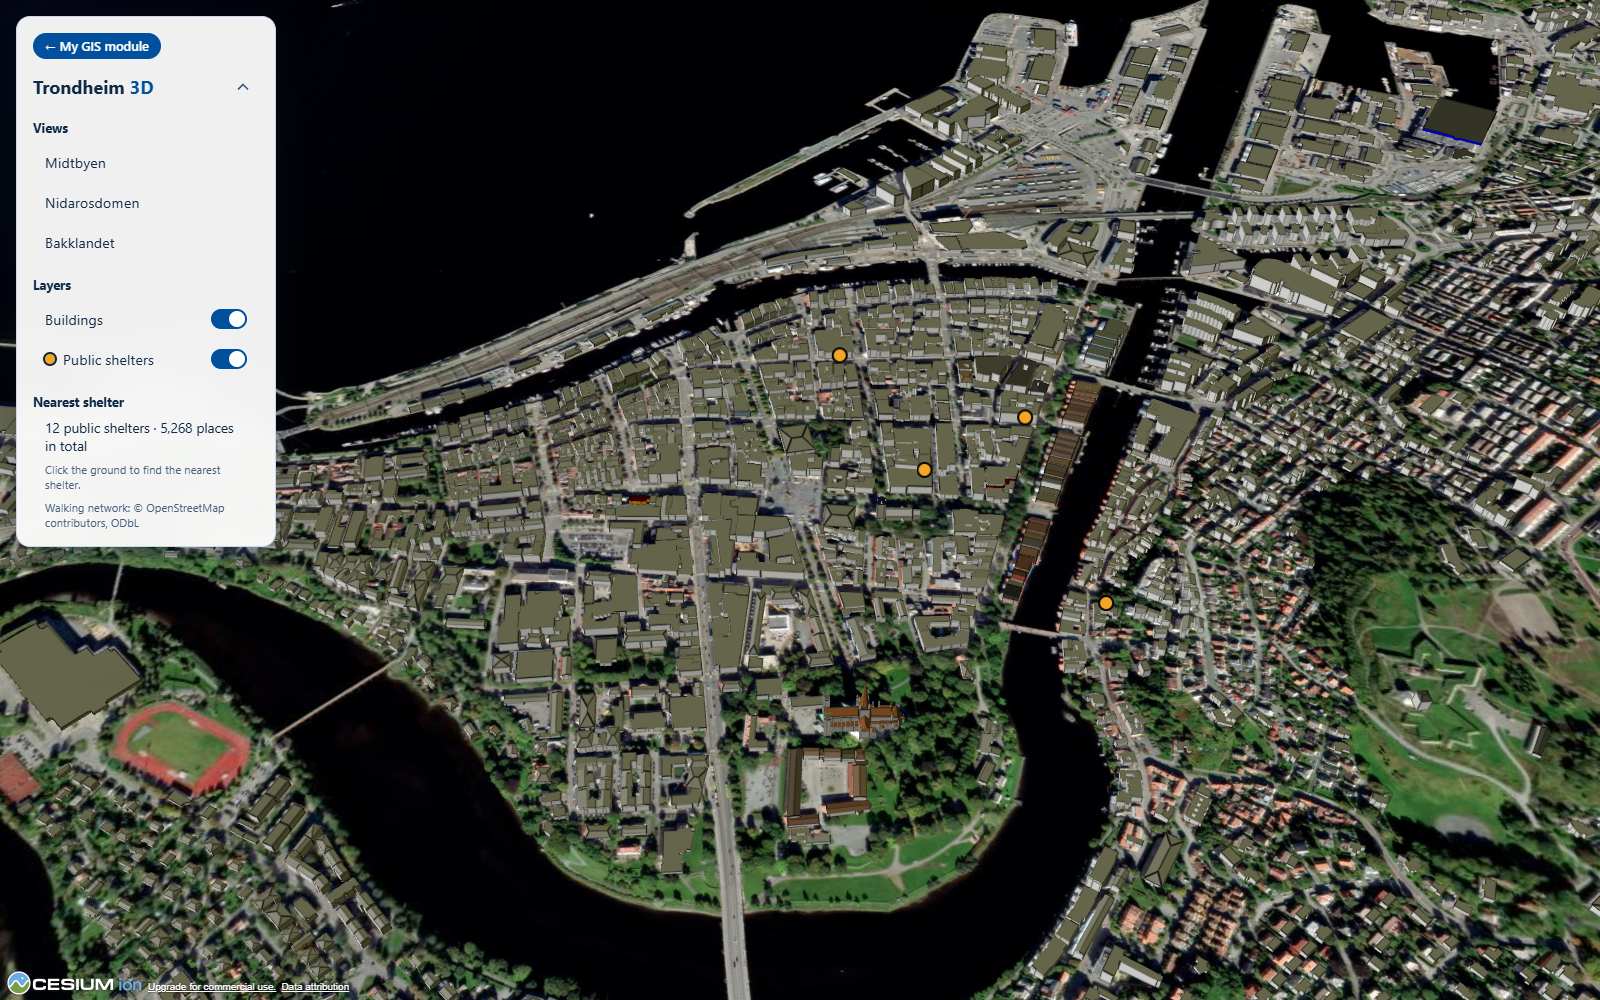
\includegraphics[width=\textwidth]{project-2-01-midtbyen-buildings.png}
\caption{Trondheim 3D: OpenStreetMap buildings on Cesium World Terrain, with the public shelters as orange points. Data: \textcopyright{} OpenStreetMap contributors (ODbL); Cesium ion; \textcopyright{} DSB (NLOD 2.0).}
\label{fig:p2-overview}
\end{figure}

\subsection{What I learned about CesiumJS}

\paragraph{The Viewer and Cesium ion.} Everything starts with a \code{Viewer}, which brings a globe, a camera and default imagery. Terrain and buildings are streamed from Cesium ion, which needs an access token. Because a web app's code is public, the token is visible to anyone; I learned to use a separate production token that only works from my own website.

\paragraph{3D Tiles.} The buildings are Cesium OSM Buildings, streamed as 3D Tiles \citep{3dtiles}: the city is split into tiles at several levels of detail, and Cesium loads finer tiles only where the camera needs them. One setting, \code{maximumScreenSpaceError}, controls this trade-off. I tested a coarser value to save memory, but small buildings in the centre disappeared, so I kept the default.

\paragraph{Entities, primitives and picking.} The shelters are \emph{entities} loaded from GeoJSON, which come with built-in selection and an info box. The buildings are a \emph{primitive}, the lower-level and faster way to draw large data. Picking showed the difference in practice: a click on a building or shelter selects that object, while a click on the ground returns a position on the terrain, which starts the nearest-shelter search.

\paragraph{The camera.} My first preset views used guessed camera positions and missed their landmarks. The fix was to describe each view as a target point plus a direction and a distance, and let Cesium place the camera in the target's local east-north-up frame. Then the landmark is always centred.

\paragraph{Using Cesium with React.} I kept Cesium code outside React components, in small modules for each layer, and gave every layer its own error handling, so the rest of the app keeps working if one dataset fails to load.

\subsection{What I learned about Norwegian geodata}

The shelters are published by DSB through an OGC Web Feature Service \citep{ogcwfs} in EUREF89 / UTM zone 32N (EPSG:25832), so they had to be converted to longitude and latitude for Cesium. Heights were the bigger lesson. Cesium measures heights above the WGS~84 ellipsoid, while Norwegian heights (NN2000) are measured above the geoid, which lies about 40\,m higher in Trondheim. Mixing the two puts a point about 40\,m too low. The walking network came from OpenStreetMap through the Overpass API \citep{overpass}.

\subsection{The nearest-shelter analysis}

Instead of a routing service, whose API key would be public in the browser, the app downloads the walking network once and searches it with Dijkstra's algorithm \citep{dijkstra1959}, directly in the browser. \Cref{fig:p2-route} shows why this matters: the nearest shelter is 490\,m away in a straight line, but the river is in the way, and the walk over Gamle Bybro is 684\,m. The analysis is simple, though: it ignores hills, stairs and how many people each shelter can take.

\begin{figure}[htbp]
\centering
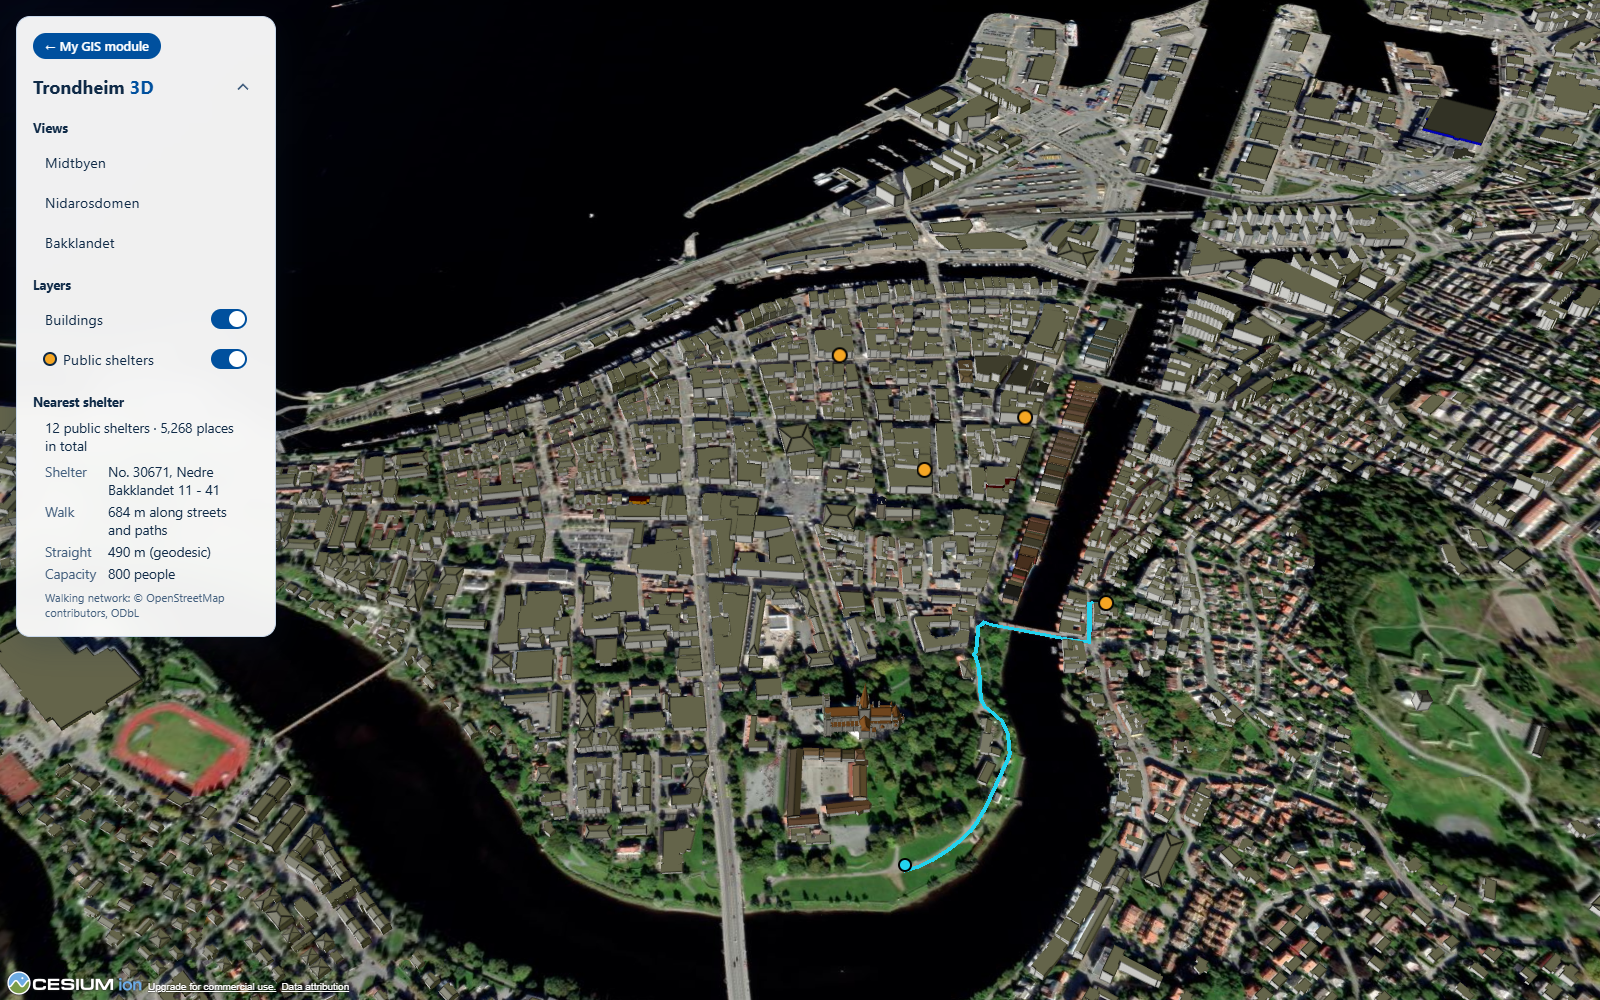
\includegraphics[width=\textwidth]{project-2-03-nearest-shelter-route.png}
\caption{A click south of Nidarosdomen: the nearest shelter is 490\,m away in a straight line, but the walk across the river is 684\,m. Data: \textcopyright{} DSB (NLOD 2.0); \textcopyright{} OpenStreetMap contributors (ODbL); Cesium ion.}
\label{fig:p2-route}
\end{figure}

\section{3DGS Viewer: learning Gaussian splatting on the web}\label{sec:p3}

\subsection{Purpose}

3D Gaussian splatting \citep{kerbl2023} is a new way to capture real places and objects in 3D from ordinary photos or video, and it is quickly showing up in GIS and digital-twin tools. I wanted to understand what a splat actually is, how it can be shown in a web browser, and what a working implementation looks like. The result is a viewer where you open your own splat file and inspect it; the file is read in the browser and never uploaded.

\paragraph{A change of plan.} The first version was a CesiumJS globe with a gallery of georeferenced splats from around the world. It turned out that the example splats only loaded with a special evaluation token from Cesium, not with my own account, and another dataset depended on a share key that expires in December 2026. A public website cannot rely on that, so I rebuilt the project as a viewer for local files. The lesson was to check data access and licences \emph{before} building on a dataset.

\subsection{What I built}

\begin{itemize}
  \item Open a splat file by dialog or drag and drop (PLY, SPZ, \code{.splat}, \code{.ksplat} or SOG).
  \item A ``file facts'' panel that reads the file header: number of splats, size, colour detail and extent.
  \item An up-axis switch and a reset button, because splat files do not agree on which way is up.
  \item A two-point distance tool.
\end{itemize}

\subsection{What I learned about Gaussian splats}

\paragraph{What a splat is.} A splat scene is a cloud of hundreds of thousands of small, semi-transparent, coloured 3D blobs (Gaussians). Each has a position, a size and orientation, an opacity and a colour that changes with the viewing angle. Unlike a mesh, there are no surfaces; unlike a point cloud, each point has a shape. The blobs are optimised so that the scene \emph{looks} right from the photos, which is why splats look so realistic.

\paragraph{What is inside the file.} Reading the PLY header myself showed that most of each record is colour: of the 59 values stored per splat in a typical file, 45 describe how the colour changes with viewing direction. This explains why splat files are large and why compressed formats such as SPZ and SOG exist.

\paragraph{Splats and GIS.} Testing with real files showed what a splat does \emph{not} contain. It has no coordinate reference system, and it does not say which way is up: the files I tested were upright with $-Y$ as up, the usual convention for 3DGS training output, but lay on their side with $+Z$, the usual convention in GIS (\cref{fig:p3-upaxis}). It also has no real scale: measuring across the lid of a jar gave 1.075 ``units'', and nothing in the file says what a unit is. To use splats in GIS, they must be georeferenced, for example with GNSS or ground control points, and can then be streamed onto a globe as 3D Tiles \citep{3dtiles,khr-gaussian-splatting}, which is what my first version tried to do.

\begin{figure}[htbp]
\centering
\begin{subfigure}{0.49\textwidth}
  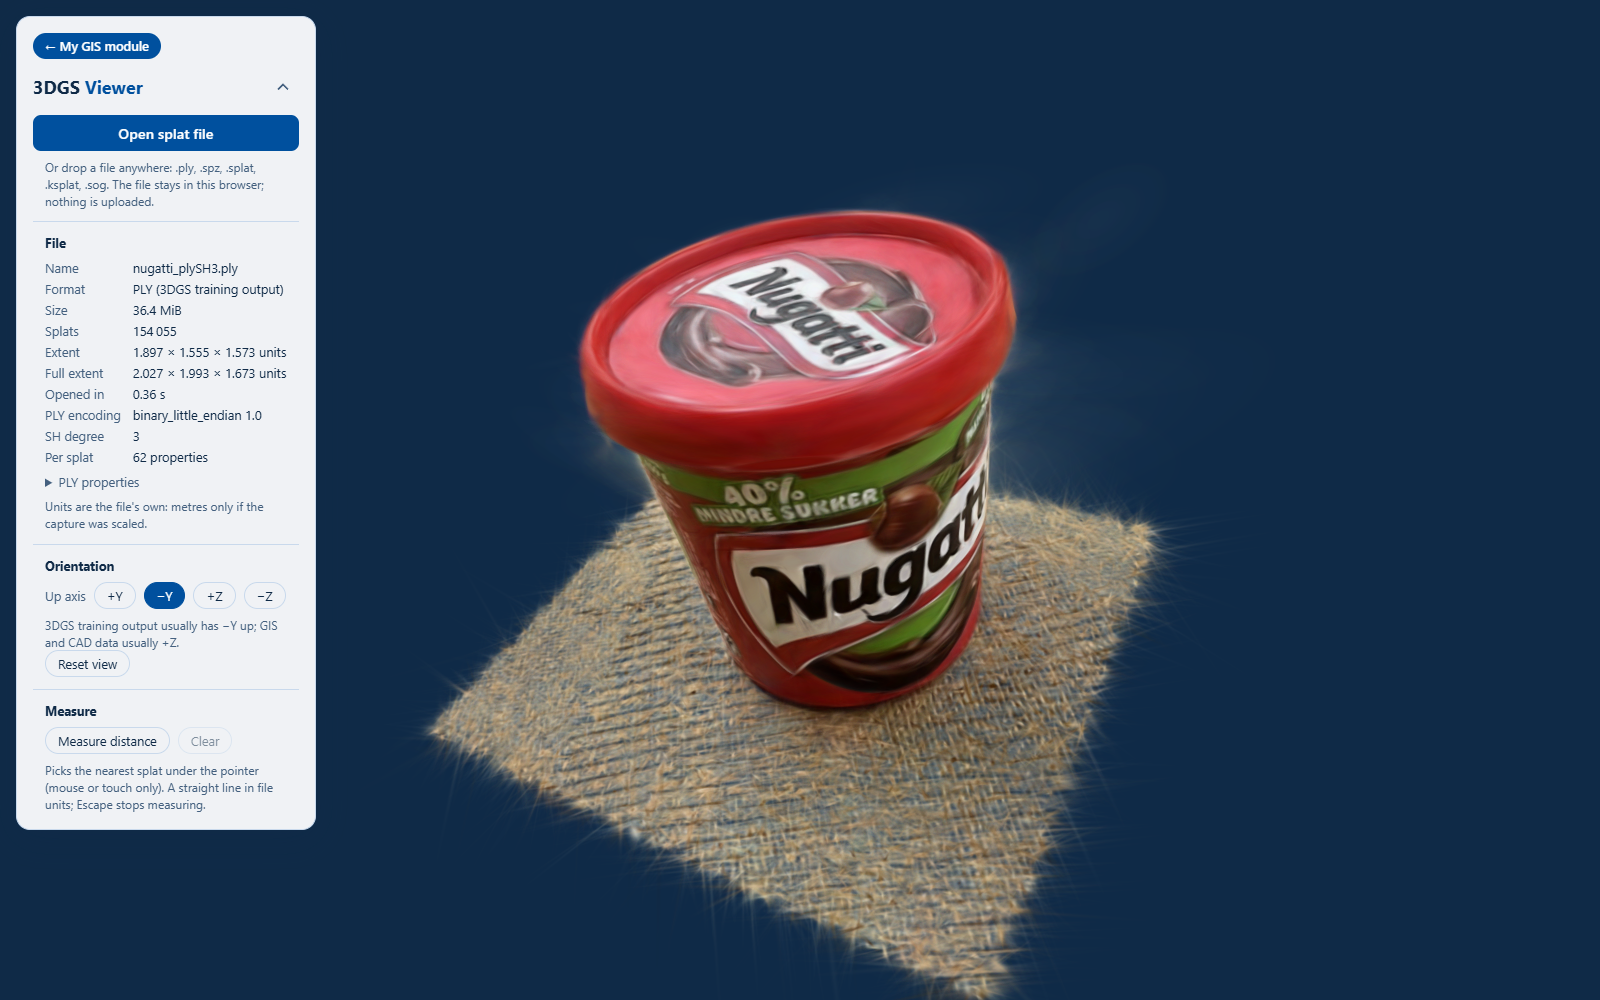
\includegraphics[width=\linewidth]{project-3-02-loaded-file-facts.png}
  \caption{Up axis $-Y$: upright}
\end{subfigure}\hfill
\begin{subfigure}{0.49\textwidth}
  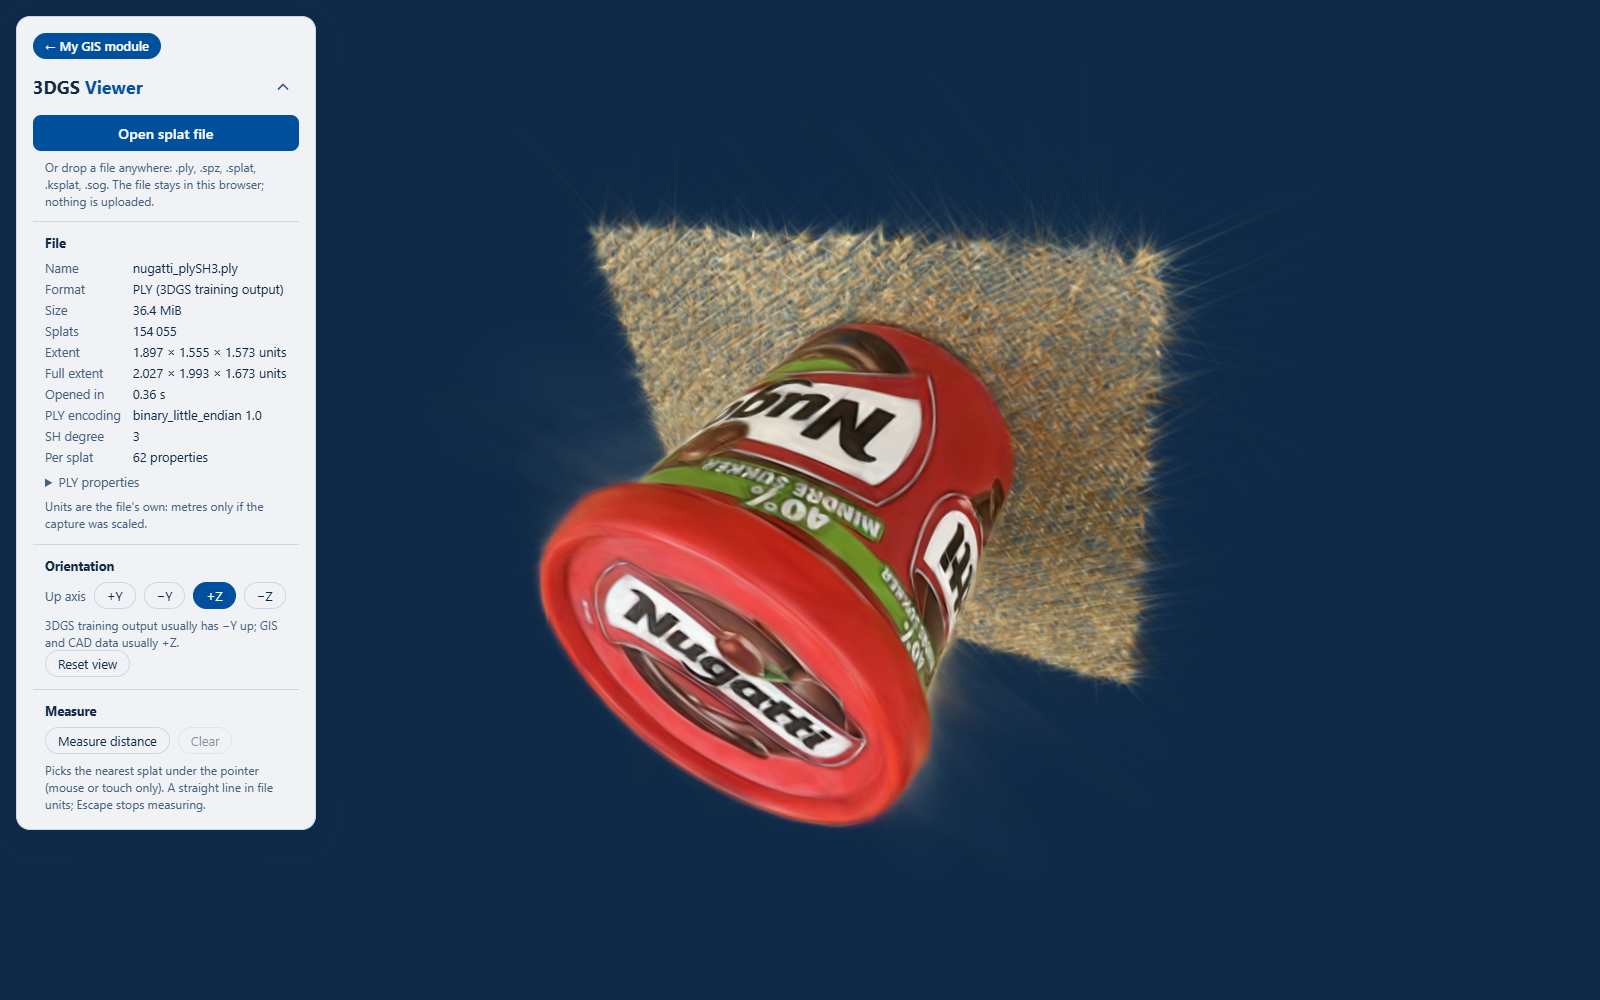
\includegraphics[width=\linewidth]{project-3-03-up-axis-wrong-plus-z.png}
  \caption{Up axis $+Z$: on its side}
\end{subfigure}
\caption{A splat of a Nugatti jar in the viewer, with the file facts in the panel. The file does not say which way is up, so the same data appears upright or on its side depending on the convention. Rendering: Spark and three.js (MIT).}
\label{fig:p3-upaxis}
\end{figure}

\subsection{What I learned about the web technology}

The viewer uses Spark \citep{spark}, a splat renderer built on three.js \citep{threejs}, the most common 3D library for the web. I learned how a three.js scene is organised (renderer, scene, camera and controls), how picking works by casting a ray from the mouse into the scene, and why the splats must be sorted by depth every time the view changes. Reading files locally, with no server or upload, keeps the app simple and private, but the renderer makes the download large before anything can be shown. Stray blobs far from the scene (``floaters'') are common in captures, so the camera is framed on the central part of the scene rather than on all splats.

\section{One website and the engineering behind it}\label{sec:website}

The three apps are built and deployed together as one static site on GitHub Pages \citep{ghpages}. A root script builds the homepage and the three apps into one folder under their paths, and one GitHub Actions workflow publishes it on every push to \code{main}. Every app uses a relative Vite \code{base} (\code{./}), so assets load under any sub-path. Projection Lab runs on Pages in its static data mode (\cref{sec:p1}). Trondheim 3D reads its Cesium ion token from a repository secret, and the production token is restricted to the Pages origin. Each project has its own CI workflow (lint, tests, build): 18 tests for Projection Lab, 54 for Trondheim 3D and 26 for the 3DGS Viewer. After the first deployment, all workflows passed, and a Playwright round trip (homepage, each app, homepage) at 1600 and 390\,px showed no console errors or failed requests (\cref{fig:mobile}).

\begin{figure}[htbp]
\centering
\begin{subfigure}{0.24\textwidth}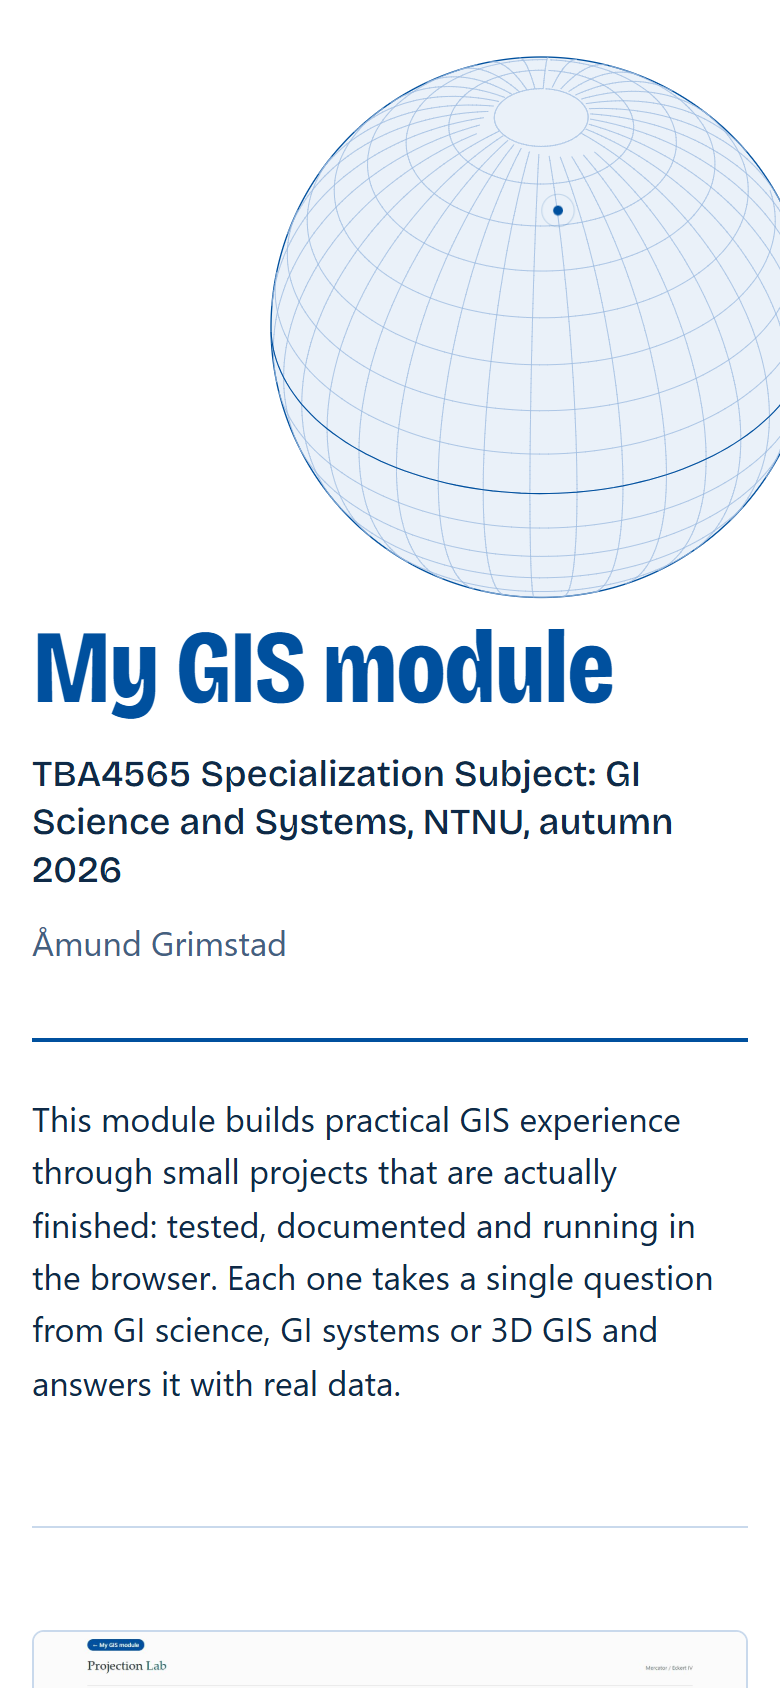
\includegraphics[width=\linewidth]{site-03-homepage-mobile.png}\caption{Homepage}\end{subfigure}\hfill
\begin{subfigure}{0.24\textwidth}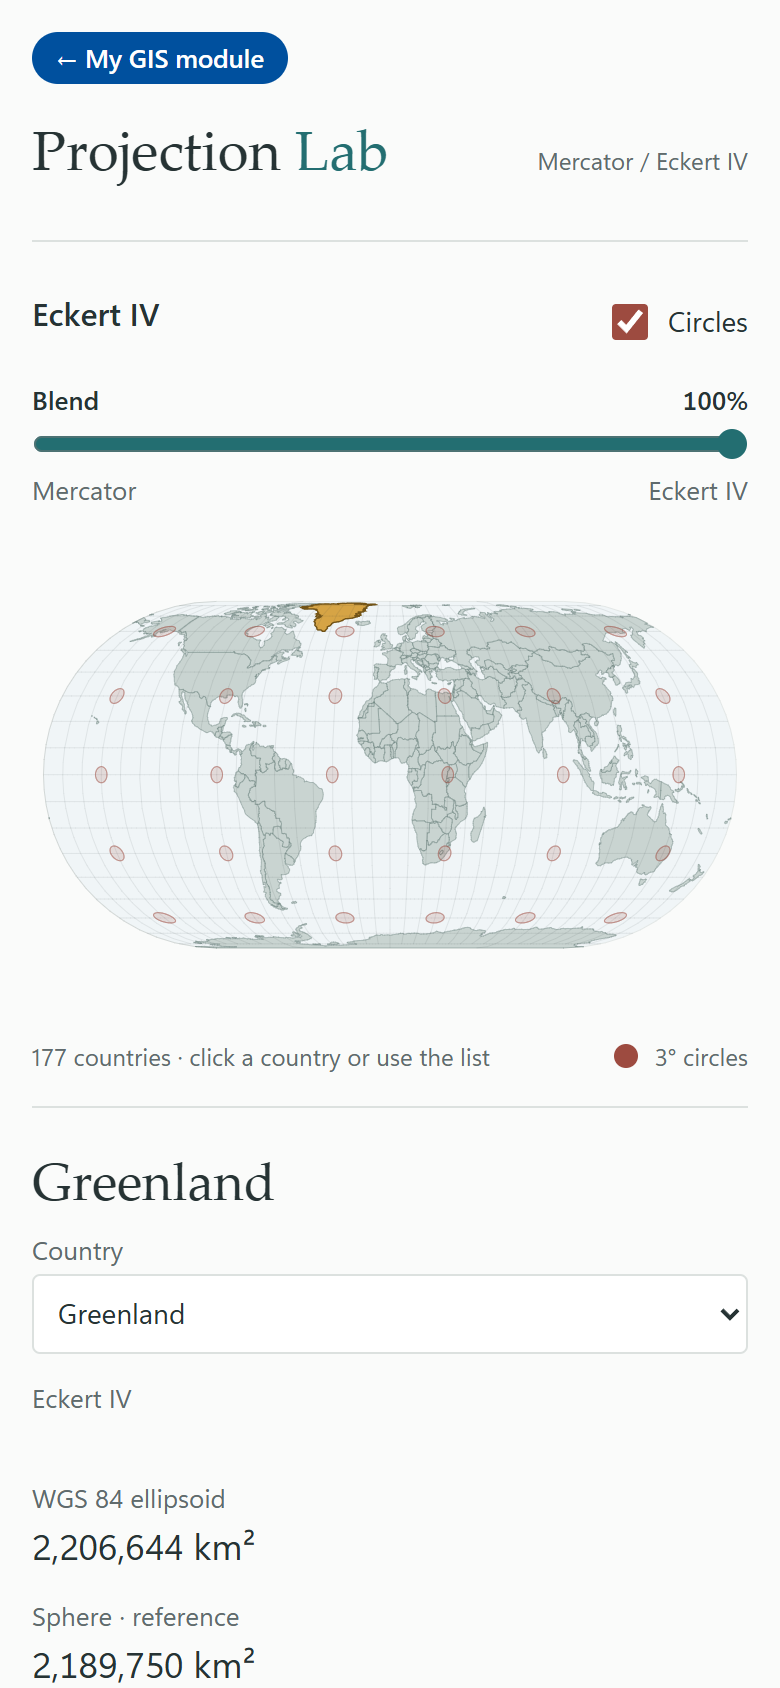
\includegraphics[width=\linewidth]{project-1-06-mobile.png}\caption{Projection Lab}\end{subfigure}\hfill
\begin{subfigure}{0.24\textwidth}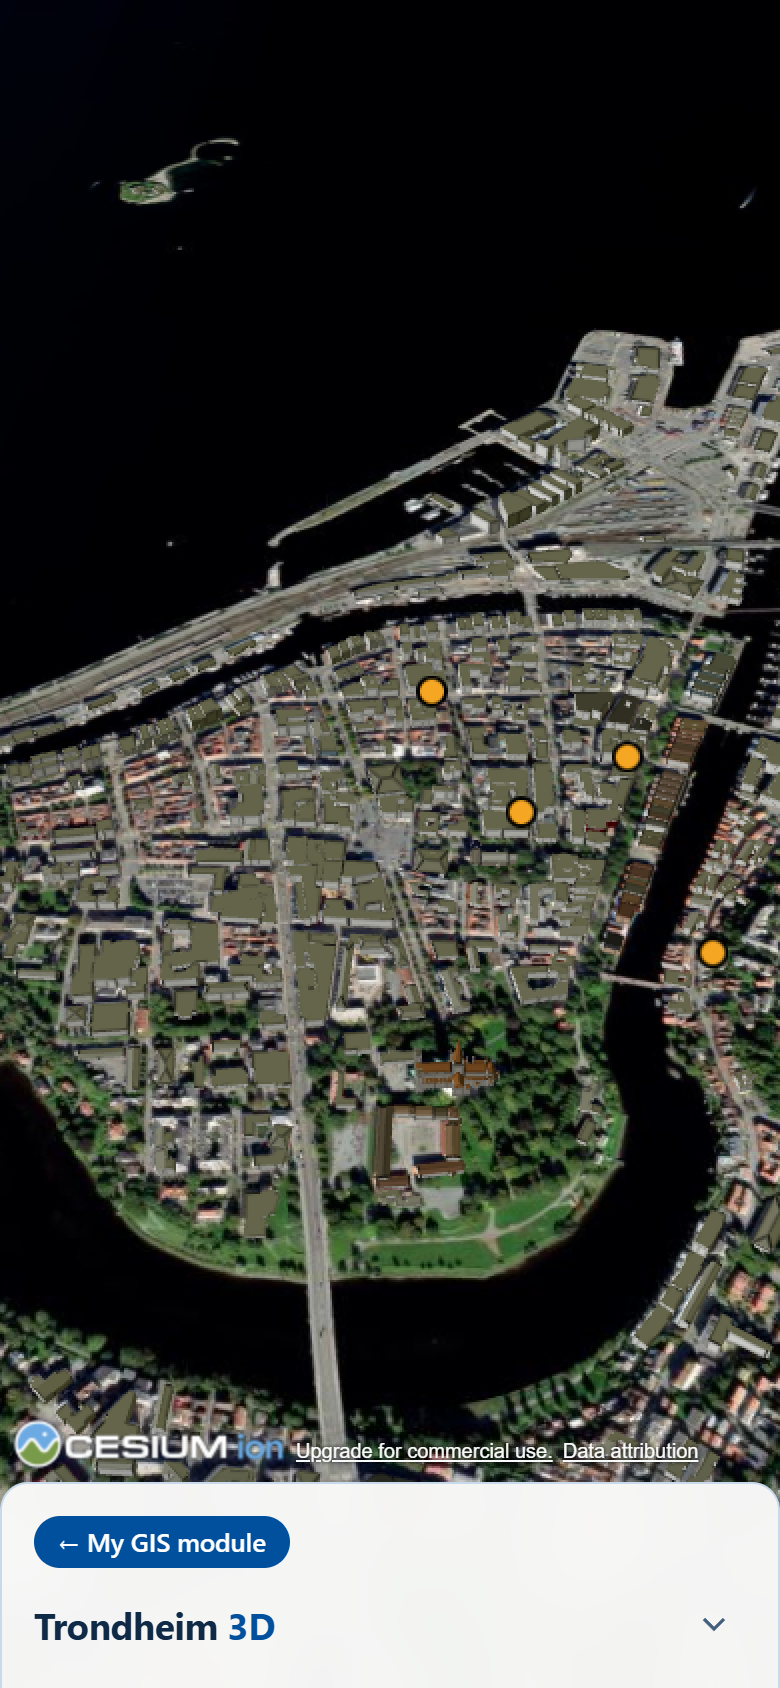
\includegraphics[width=\linewidth]{project-2-04-mobile.png}\caption{Trondheim 3D}\end{subfigure}\hfill
\begin{subfigure}{0.24\textwidth}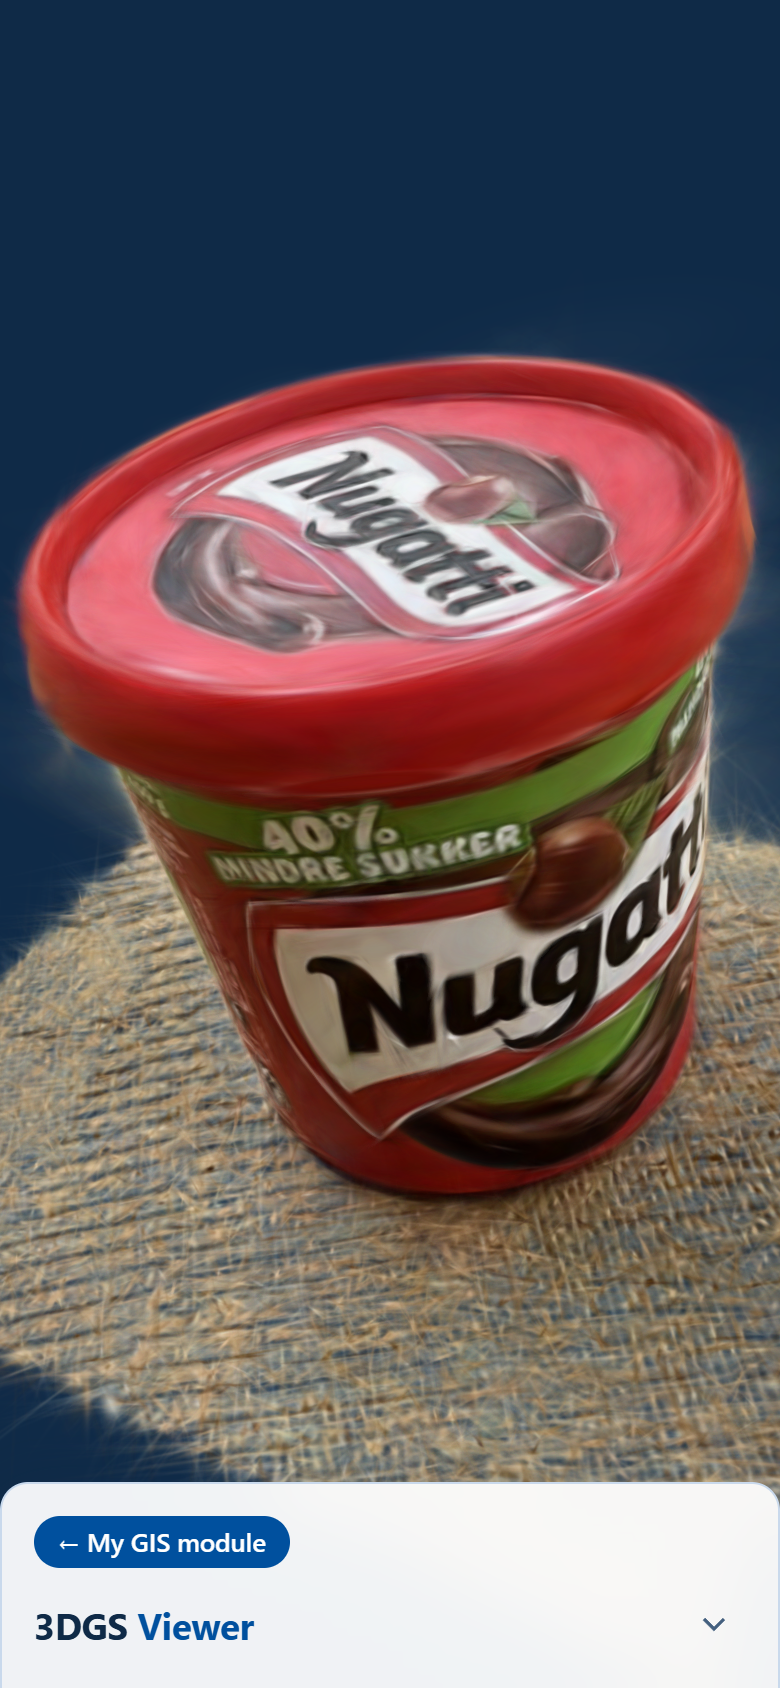
\includegraphics[width=\linewidth]{project-3-05-mobile.png}\caption{3DGS Viewer}\end{subfigure}
\caption{The site at phone width (390\,px). Each app links back to the homepage. Data: Natural Earth; \textcopyright{} OpenStreetMap contributors (ODbL); \textcopyright{} DSB (NLOD 2.0); Cesium ion.}
\label{fig:mobile}
\end{figure}

\section{Discussion}\label{sec:discussion}

% TODO (author): expand this reflection in your own words.
The three projects cover the three themes of the course from different angles. Projection Lab is GI science: a theoretical result ($\sec^2\varphi$ and Jensen's inequality) tested against measurement. Trondheim 3D is GI systems: most of its value lies in combining reference systems, data sources and services, and its analysis shows that a straight-line answer points to the wrong shelter at about one location in five. The 3DGS Viewer shows how far a popular new 3D data type still is from GIS use: without georeferencing it has no CRS, no reliable up direction and no scale.

Working with an AI coding assistant made the projects larger than I could have built alone, but it moved the work from writing code to directing and checking it. The most useful habits were to write the rules down (no invented numbers, verify before claiming), to require a runnable check for every change, and to inspect the screenshots myself. The pivot of the 3DGS project also showed the value of checking data access and licences before building on a dataset.

\section{Conclusion}\label{sec:conclusion}

Mercator inflates the median country area by $1.21\times$ and Greenland by $16.54\times$, and $\sec^2\varphi$ at the centroid predicts the inflation within 1\,\% for 156 of 176 countries while never overestimating it. In central Trondheim, the nearest public shelter on foot differs from the nearest in a straight line at 19\,\% of reachable grid points, and the median walk is 1.34 times the straight line. A Gaussian splat file can be opened and inspected entirely in the browser, but it carries no reference system, up direction or scale. All three apps are tested, documented and live at \siteurl.

\appendix
\section{Reproducing the results}\label{app:repro}

From the repository root (Windows PowerShell, Node 24, Python 3.14 with uv): \code{uv run --locked --project "Project 1/backend" pytest}; \code{npm --prefix "Project 2" test} and \code{npm --prefix "Project 3" test} (plus \code{run lint} and \code{run build}); the whole website with \code{npm run site:install} and \code{npm run site:build}. The Projection Lab database stack is described in \code{Project 1/README.md}.

\section{Data credits and licences}\label{app:credits}

Country boundaries: Natural Earth (public domain). Buildings and walking network: \textcopyright{} OpenStreetMap contributors (ODbL). Public shelters: \textcopyright{} DSB (NLOD 2.0). Terrain, imagery and 3D Tiles streaming: Cesium ion. Camera-target heights: Kartverket (CC BY 4.0). SOAR Telescope splat: Luis Cerda (CC BY 4.0). Splat rendering: Spark and three.js (MIT).


\bibliographystyle{plainnat}
\bibliography{references}

\end{document}
